\documentclass[11pt,a4paper,titlepage,leqno]{article}
\usepackage[utf8]{inputenc}
\usepackage{listings}
\usepackage{amsmath}
\usepackage{amsfonts}
\usepackage{amssymb}
\usepackage{makeidx}
\usepackage{graphicx}
\usepackage{color}
\usepackage{tikz-qtree}
\usepackage{float}
\usepackage{paralist}

\title{Optimizacion de Consultas: Informe}
\author{Juan Pablo Civile \and Martin Sturla}
\date{13 de Noviembre de 2012}


\newcommand{\pr}[2]{\Pi_{#1}(#2)}
\newcommand{\join}[2]{#1 \bowtie #2}
\newcommand{\filter}[2]{\sigma_{#1}(#2)}
\newcommand{\ejercicio}[1]{
    \section*{Ejercicio #1}
    \setcounter{answer}{0}
}

\newcounter{answer}
\newcommand{\answer}{
    \addtocounter{answer}{1}
    \arabic{answer}.
}

\newcommand{\equ}[1]{
    \subsection*{\answer}
    \begin{equation}
        \tag*{}
        #1
    \end{equation}
}

\newcommand{\parte}{
    \subsection*{\answer}
}

\lstset{
    language = SQL,
    basicstyle=\footnotesize
}


\begin{document}

\maketitle

\ejercicio{1}

saayyyyyyyyyyyyyyyy waaaaaaaaaaaaaaaaaaaaaaaaaaaaaaaaaaaaaaaaaaaaaaaaaaaaaat

\ejercicio{2}

\parte
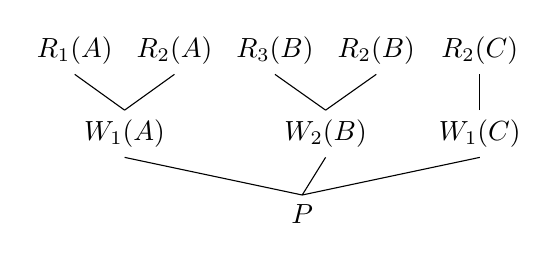
\begin{tikzpicture}[grow'=up]
    \Tree [. {$P$}
        [. {$W_1(A)$}
            [. {$R_1(A)$} ]
            [. {$R_2(A)$} ]
        ]
        [. {$W_2(B)$}
            [. {$R_3(B)$} ]
            [. {$R_2(B)$} ]
        ]
        [. {$W_1(C)$}
            [. {$R_2(C)$} ]
        ]
    ]
\end{tikzpicture}

\parte

\begin{inparaenum}[]
    \item $R_3(B)$
    \item $R_2(A)$
    \item $R_2(C)$
    \item $R_2(B)$
    \item $W_2(B)$
    \item $R_1(A)$
    \item $W_1(A)$
    \item $W_1(C)$
\end{inparaenum}

\parte

Insufficient data.

\ejercicio{3}

No sigue las reglas de \textit{2PL Estricto}, ya que no sigue las reglas basicas de \textit{2PL}. $T_2$ libera el lock que tiene sobre $A$ antes de tomar un lock sobre $B$, que no se permite en \textit{2PL}.

\ejercicio{4}

\parte

Hay 9 planes posibles.

\parte

Solo un plan.

\ejercicio{5}

Si consideramos las posibilidades sin contar las operaciones \texttt{START} y \texttt{COMMIT}, solo 4 planes son posibles. Uno es el plan serial $(T_1, T_2)$, otro (
\begin{inparaenum}[]
    \item $R_1(A)$,
    \item $R_1(B)$,
    \item $INC_1(A)$,
    \item $R_2(A)$,
    \item $INC_1(B)$,
    \item $R_2(B)$,
    \item $INC_2(A)$,
    \item $INC_2(B)$
\end{inparaenum}
), y los ultimos 2 planes son iguales excepto que es invierte $T_1$ por $T_2$.

Para los alternativas seriales hay 36 posibles planes dependendiendo de la ubicacion de \texttt{START} y \texttt{COMMIT}, y para las otras alternativas son 25 posibles planes. Eso nos deja con un total de 124 planes.

\ejercicio{6}

Solo una operacion es posible, $R_2(C)$.

\ejercicio{7}

$2^9$. Las operaciones no son conflictivas, y con el uso de shared locks pueden ocurrir en cualquier orden sin demoras.

\ejercicio{8}



\end{document}
